%% -*- coding:utf-8 -*-

\documentclass[output=paper
  ,nobabel
  ,draftmode
  ,colorlinks, citecolor=brown
]{langscibook}


\IfFileExists{../localcommands.tex}{%hack to check whether this is being compiled as part of a collection or standalone
   \usepackage{orcidlink}

% add all extra packages you need to load to this file


% Haitao Liu
%\usepackage{xeCJK}
%\setCJKmainfont{SimSun}
%\setCJKmainfont[Scale=MatchUppercase,
%                Path=fonts/
%]{SourceHanSerifSC-Regular}

% instead use option:  ,chinesefont % for references in raffelsiefen.tex
% loading the package changes some spacings


\usepackage{multicol}
\usepackage{tikz}\usetikzlibrary{decorations.pathreplacing}
\usepackage{url}
\urlstyle{same}

%\usepackage{listings}
%\lstset{basicstyle=\ttfamily,tabsize=2,breaklines=true}

\usepackage{langsci-basic}
\usepackage{langsci-optional}
\usepackage[danger]{langsci-lgr}

% toggle danger in texlive 2021
%\newcommand{\M}{\textsc{m}\xspace}

% toggle danger in texlive 2021 or uncomment this
% \newcommand{\N}{\textsc{n}\xspace}
% \newcommand{\F}{\textsc{f}\xspace}


\usepackage{./styles/biblatex-series-number-checks}




\usepackage{langsci-gb4e}




% Demske

\usepackage{tipa}
\usepackage{styles/avm+}
%\usepackage{styles/merkmalstruktur}
\avmfont{\sc}
\usepackage{langsci-forest-setup}
\usepackage{xspace}
%\usepackage{styles/abbrev} 

\usepackage{soul}
\usepackage{color}
\newcommand{\rem}[1]{\textcolor{red}{\st{#1}}}
\newcommand{\add}[1]{\textcolor{blue}{\ul{#1}}}


% Salzmann

\usepackage[nocenter]{qtree}


% Müller

% add this to the default preamble 
\forestset{default preamble={
    for tree={anchor=north},
}}


\usepackage{german}

%\usepackage{german}
\selectlanguage{USenglish}

% Mit Babel geht irgendwie die hyphenation nicht richtig
%\usepackage[ngerman,english]{babel}
%\useshorthands{"} 
%\addto\extrasenglish{\languageshorthands{ngerman}}

\usepackage{styles/makros.2020,
styles/abbrev,
styles/merkmalstruktur,
styles/article-ex,styles/eng-date}


\usepackage{todonotes}
\newcommand{\todostefan}[1]{\todo[color=green!40]{\footnotesize #1}\xspace}
\newcommand{\inlinetodo}[1]{\todo[color=green!40,inline]{\footnotesize #1}\xspace}

\newcommand{\inlinetodoopt}[1]{\todo[color=green!40,inline]{\footnotesize #1}\xspace}
\newcommand{\inlinetodoobl}[1]{\todo[color=red!40,inline]{\footnotesize #1}\xspace}

\newcommand{\itdobl}[1]{\inlinetodoobl{#1}}
\newcommand{\itdopt}[1]{\inlinetodoopt{#1}}

\newcommand{\addpages}{\todostefan{add pages}}

%\newcommand{\iaddpages}{\yel[add pages]{pages}\xspace}



% subfigure
\usepackage{subcaption}



% Nolda
%\usepackage[main=british,nil,german,french]{babel}
\newcommand{\foreignlanguagedummy}[2]{#2}
\usepackage{tagpair}
\usepackage{hang}
\usepackage[noconfig]{ntheorem}
\usepackage{pstricks,pst-node,pst-tree}
\usepackage{newunicodechar}



   \newcommand*{\orcid}[1]{}

% do not show the chapter number. It is redundant, since most references to figures are within the
% same chapter.
\renewcommand{\thefigure}{\arabic{figure}}

\newcommand{\rlapsub}[1]{\rlap{\sub{#1}}}

% \SetupAffiliations{output in groups = false, 
%                    separator between two = {\bigskip\\},
%                    separator between multiple = {\bigskip\\},
%                    separator between final two = {\bigskip\\}
%                    }


%%%%%%%%Alte Umlaute
\newcommand{\oldae}{$\stackrel{\textrm{\tiny e}}{\textrm{a}}$}
\newcommand{\oldoe}{$\stackrel{\textrm{\tiny e}}{\textrm{o}}$}
\newcommand{\oldue}{$\stackrel{\textrm{\tiny e}}{\textrm{u}}$}

\newcommand{\refl}{\REFL}
\newcommand{\pst}{\PST}


% Müller
\let\vref\ref


\let\citew\citet

\newcommand{\page}{}

% biblatex stuff
% get rid of initials for Carl J. Pollard and Carl Pollard in the main text:
\ExecuteBibliographyOptions{uniquename=false}




\newcommand{\nom}{\textsc{nom}}
\newcommand{\gen}{\textsc{gen}}
\newcommand{\dat}{\textsc{dat}}
\newcommand{\acc}{\textsc{acc}}


%\newcommand{\spacebr}{\hspaceThis{[}}



\newcommand{\acknowledgmentsEN}{Acknowledgements}
\newcommand{\acknowledgmentsUS}{Acknowledgments}


% no bf!!!111!
\let\textbfemph\emph

\newcommand{\textbfremoved}[1]{#1}
%\newcommand{\emphremoved}[1]{#1}


\newcommand{\noemph}[1]{#1}
\newcommand{\underlineemph}[1]{\emph{#1}}




% for editing, remove later
\usepackage{xcolor}
\newcommand{\added}[1]{{\red #1}}
\newcommand{\addedthis}{\todostefan{added this}}

\newcommand{\changed}[1]{\textcolor{orange}{#1}}




% Nolda

\theorembodyfont{\normalfont}
\let\restriction\relax
\renewtheoremstyle{break}{\item{\itshape ##1\ ##2}\newline\nopagebreak}{\item{\itshape ##1\ ##2\ (##3)}\newline\nopagebreak}
\theoremstyle{break}
\newtheorem{definition}{Definition}
\newtheorem{pattern}{Pattern}
\newtheorem{restriction}{Restriction}
\newunicodechar{‑}{\hbox{-}}
\newunicodechar{…}{\dots}
\newunicodechar{⁡}{\relax}
\newunicodechar{⁣}{\relax}
\newunicodechar{⁀}{\raisebox{+1ex}{\ensuremath\frown}}
\newunicodechar{⁐}{\raisebox{+1ex}{\ensuremath\frown}\setbox1=\hbox{\ensuremath\smile}\hspace{-\wd1}\raisebox{-1ex}{\ensuremath\smile}}
\newunicodechar{⪪}{\ensuremath{<\mathrel{\llap{\ensuremath{-}}}}}
\setkomafont{descriptionlabel}{\normalfont}
\ExecuteBibliographyOptions{labeldate=comp,labelnumber=true,defernumbers=true}
\defbibenvironment{sources}{\list{\printfield{labelprefix}\,\printfield{labelnumber}}{\settowidth{\labelwidth}{S\,0}\setlength{\labelsep}{\biblabelsep}\setlength{\leftmargin}{\labelwidth}\addtolength{\leftmargin}{\labelsep}\setlength{\itemsep}{\bibitemsep}\setlength{\parsep}{\bibparsep}}\renewcommand{\makelabel}[1]{##1\hfil}}{\endlist}{\item}
\newcommand{\citesource}[1]{\citefield{#1}{labelprefix}\,\citefield{#1}{labelnumber}}


% Was soll das machen?
\newcommand{\textstyleFootnoteSymbol}{}



% Was ist das???? St. Mü. 30.10.2021
%Kann weg. Damit waren die bücker transkripte aligniert. Habe das jetzt mit tabularx und hphantom gemacht

%\newlength{\calength} %tmp length to store the space 1. until [; 2. until ].
%
%%first argument speaker ID, second argument text. Optional argument left margin indicator (arrow or similar)
%\newcommand{\cabox}[3][]{\parbox{0mm}{\hspace*{-1cm}#1}%
%\parbox{1.5cm}{#2}%
%\parbox{9.6cm}{#3}\\%
%}
%
%%translation. First parbox is empty, second parbox takes the translation text
%\newcommand{\trsbox}[1]{\parbox{1.5cm}{~}%
%\parbox{9.6cm}{\itshape #1}\\%
%}
%
%%store the width of a string.
%\newcommand{\settablength}[1]{\settowidth{\calength}{#1}\global\calength=\calength}
%
%%print string and store its width. Useful if the first item of the aligned set is also the longest
%\newcommand{\inittab}[1]{#1\settablength{#1}}
%
%%insert horizontal white space equivalent to the stored width
%\newcommand{\skiptab}{\parbox{\calength}{~}}
%
%%print the argument and fill up with horizontal white space until the stored width is reached.
%\newcommand{\filledtab}[1]{\parbox{\calength}{#1}}



% for standalone compilations Felix: This is in the class already
%\let\thetitle\@title
%\let\theauthor\@author 
\makeatletter
\newcommand{\togglepaper}[1][0]{ 
\bibliography{../bib-abbr,../stmue,../localbibliography,
collection.bib}
  %% hyphenation points for line breaks
%% Normally, automatic hyphenation in LaTeX is very good
%% If a word is mis-hyphenated, add it to this file
%%
%% add information to TeX file before \begin{document} with:
%% %% hyphenation points for line breaks
%% Normally, automatic hyphenation in LaTeX is very good
%% If a word is mis-hyphenated, add it to this file
%%
%% add information to TeX file before \begin{document} with:
%% \include{localhyphenation}
\hyphenation{
Arsch
anaph-o-ra
Bü-cking
con-stit-u-ents
Dor-drecht
For-schungs-ge-mein-schaft
Ge-schich-te
ha-ben
pho-nol-o-gy
pro-so-dic
pro-so-di-cally
Sal-pe-ter
sei-nen
Wil-liams
}
\hyphenation{
Arsch
anaph-o-ra
Bü-cking
con-stit-u-ents
Dor-drecht
For-schungs-ge-mein-schaft
Ge-schich-te
ha-ben
pho-nol-o-gy
pro-so-dic
pro-so-di-cally
Sal-pe-ter
sei-nen
Wil-liams
}
  % \memoizeset{
  %   memo filename prefix={hpsg-handbook.memo.dir/},
  %   % readonly
  % }
  \papernote{\scriptsize\normalfont
    \@author.
    \titleTemp. 
    To appear in: 
    Ulrike Freywald \& Horst Simon (eds.) Headedness and/or grammatical anarchy?
    Berlin: Language Science Press. [preliminary page numbering]
  }
  \pagenumbering{roman}
  \setcounter{chapter}{#1}
  \addtocounter{chapter}{-1}
}
\makeatother



% This does a linebreak for \gll for long sentences leaving space for the language at the right
% margin. The factor .0989 is needed since otherwise starred examples cause a linebreak.
% St.Mü. 17.06.2021 08.02.2021
\newcommand{\longexampleandlanguage}[2]{%
%\begin{tabularx}{.99\linewidth}[t]{@{}X@{}p{\widthof{(#2)}}@{}}%
%\begin{minipage}[t]{.99\linewidth}%
\begin{tabularx}{\linewidth}[t]{@{}X@{}p{\widthof{(#2)}}@{}}%
\begin{minipage}[t]{\linewidth}%
#1%
\end{minipage} & (\ili{#2})%
\end{tabularx}}

% ORCIDs in langsci-affiliations 
\usepackage{orcidlink}
\definecolor{orcidlogocol}{cmyk}{0,0,0,1}
\ProvideDocumentCommand{\LinkToORCIDinAffiliations}{ +m }
  {%
    \orcidlink{#1}
  }

   %% hyphenation points for line breaks
%% Normally, automatic hyphenation in LaTeX is very good
%% If a word is mis-hyphenated, add it to this file
%%
%% add information to TeX file before \begin{document} with:
%% %% hyphenation points for line breaks
%% Normally, automatic hyphenation in LaTeX is very good
%% If a word is mis-hyphenated, add it to this file
%%
%% add information to TeX file before \begin{document} with:
%% %% hyphenation points for line breaks
%% Normally, automatic hyphenation in LaTeX is very good
%% If a word is mis-hyphenated, add it to this file
%%
%% add information to TeX file before \begin{document} with:
%% \include{localhyphenation}
\hyphenation{
Arsch
anaph-o-ra
Bü-cking
con-stit-u-ents
Dor-drecht
For-schungs-ge-mein-schaft
Ge-schich-te
ha-ben
pho-nol-o-gy
pro-so-dic
pro-so-di-cally
Sal-pe-ter
sei-nen
Wil-liams
}
\hyphenation{
Arsch
anaph-o-ra
Bü-cking
con-stit-u-ents
Dor-drecht
For-schungs-ge-mein-schaft
Ge-schich-te
ha-ben
pho-nol-o-gy
pro-so-dic
pro-so-di-cally
Sal-pe-ter
sei-nen
Wil-liams
}
\hyphenation{
Arsch
anaph-o-ra
Bü-cking
con-stit-u-ents
Dor-drecht
For-schungs-ge-mein-schaft
Ge-schich-te
ha-ben
pho-nol-o-gy
pro-so-dic
pro-so-di-cally
Sal-pe-ter
sei-nen
Wil-liams
}
    \bibliography{localbibliography}
    \togglepaper[23]
}{}


\title[Anarchy in Grammar?]{Anarchy in Grammar? On headedness and some of its problems, illustrated by examples from German} 
\ChapterDOI{10.5281/zenodo.7142615}

\author{Ulrike Freywald\orcid{0000-0003-3268-7874}\affiliation{TU Dortmund} and Horst J. Simon\orcid{0000-0002-6367-2969}\affiliation{Freie Universität Berlin}}
% \chapterDOI{} %will be filled in at production

% \epigram{}

\abstract{One of the fundamental characteristics of grammars of human languages seems to be the fact that (most of) their structures are inherently asymmetric, with exactly one element, the \emph{head}, being more important than its co-elements. By way of introduction to this volume, we discuss some phenomena that pose potential problems for such a view and that have not yet been fully described empirically and understood theoretically. Here we focus on three structures from German, namely ``left-headed'' (?) verbs, then morphological reduplications and copulative/""coordinative compounds, and finally (auxiliary) verb ellipses, all of which are not easily captured by a straightforward analysis in terms of head structures. }


\begin{document}

\maketitle

\section{Grammar is all about hierarchies, or maybe not? – Structure-building in grammar}

\largerpage
Once you start thinking about it, it appears that Grammar is a rather unlikable thing: it is full of
asymmetries, full of dependencies, full of hierarchies.\footnote{Fortunately we also have agreement
  and harmony and the like.} Why is that so?\footnote{The following reasoning is of course a gross
  simplification, but the general idea should hopefully become clear.} – Now, if you imagine a
completely blank slate with regard to grammatical modelling (on the part of the linguist; or with
regard to grammatical knowledge if you consider a new-born baby) the situation might be described
like this: In the beginning there is just noise; the speech signal you receive consists of seemingly
unstructured sounds.\footnote{This is similar to the situation one experiences when one hears an
  entirely unknown language.} However, you will soon realise that certain elements stick out:
syllables with their vocalic nuclei, certain syllables that are more accentuated than others (in
most languages) etc. In other words, a major factor to be taken into account when describing a
language is `prominence', the fact that some elements are more conspicuous and thus also somehow
more important than others.

You will also realise that certain sound combinations co-occur together time and again, that's what
linguists call \emph{words}, or sometimes larger units, collocations. In many languages, these
words sometimes occur with minor differences, i.e. modifications or further elements added to them:
inflection. After a while you will realise that not only sounds regularly co-occur in order to form
words, but also that some of those words tend to come together with specific other words, or at
least with one or another word of a small group of other words. In other words, words can be grouped
into classes. The members of these classes share certain commonalities; for instance, members of one
class tend to be preceded – immediately or with something in-between – by elements from another word
class. Thus we get a distinction between, say, nouns and articles in \ili{English} or \ili{German} or \ili{French}. If
you carry out such classificatory operations long enough, by determining (types of) elements that
somehow hang together, you will gradually build up a system of the building blocks of a language:
sounds, words, and what in many grammatical models is called phrases. In their entirety, all these
elements constitute a complex network of interrelations.

Interestingly now, not all of these elements are of equal standing with regard to their interaction
with other elements, that is with regard to their behaviour in larger linguistic structures, the way
they fit into those units. Some elements seem to be more important for structure-building at a
particular location in the system than others. Factors that are relevant for the relative importance
of elements include: the degree of obligatoriness of their occurrence within a particular structure,
their ability to determine the occurrence and even the particular shape of other elements nearby,
their ability to determine certain properties of the whole group of elements in which they occur.

So, for example, and like before we simplify slightly, in certain structures a verb is (more or
less) certainly there – otherwise the whole thing would be a different structure altogether; such a
verb, by virtue of its valency, requires through a dependency relation the presence of certain other
elements (called arguments, i.e. a subject, potentially also objects) and can assign them a
particular case; all structures combining such an element \emph{verb} with its companion(s) are
verb phrases and share certain properties. For example, in most grammatical structures in languages
such as \ili{English} or \ili{German} verbs have endings that indicate different \emph{tenses}, and this
entails that at some higher level the whole group containing the verb will have
tense.\footnote{Needless to say for linguists, depending on the particular grammatical framework you
  happen to work in, you might believe that things are much more complicated, such that, strictly
  speaking, it is not the verb phrase in the narrow sense that is tensed, but a somewhat more subtle
  grammatical element called the Inflectional Phrase or Tense Phrase or some other superordinated
  structural element or feature, respectively.}  To put it in a nutshell: a verb phrase is a verb
phrase only by virtue of its containing an obligatory element called verb, which is thus its most
important element and which exhibits certain (combinatorial) properties, which in turn influence
some of the properties of the structure at large, for instance how many verbal arguments this
structure contains.

Such reasonings can be generalised: similar structure-building processes seem to occur at all levels
of grammar, from phonology through morphology to syntax. We will always find structures where some
element is more central, more dominant, more important than the other. This very observation is, of
course, the rationale behind the wide-spread application of a notion \emph{head} in grammatical
theorising, in theorising across widely different grammatical models. Thus, the classical literature
on the subject (since \citealt{Bloomfield1933}) has collected a variety of characteristics of
grammatical heads (in contrast to non-heads) that they exhibit typically in their respective
structures:\footnote{We need to list only the most important publications here: \citet{Lieber1981},
  \citet{Williams1981}, \citet{Selkirk1982}, \citet{Zwicky85a}, \citet{Hudson1987},
  \citet{CorbettEtAl1993}, \citet{Croft1996}, among many others.} Usually, heads are obligatory,
determine the category and other properties of the structure they are part of, select for elements
they co-occur with, and determine features of their respective non-heads via agreement, case and
theta-role assignment, etc. – However, not all grammatical structures can be easily captured with
such a notion of head: Time and again we find exceptional structures where there either seems to be
no head at all because there is no structural asymmetry involved or where there seems to be a head
that exerts some influence, but stays invisible otherwise, or where there is a head that just
behaves in an unexpected way, for example by occurring in the “wrong'' position with regard to the
language-specific serialisation rules.\footnote{For a general discussion of how grammatical
  exceptions can be dealt with theoretically cf., e.g., \citet{SimonWiese2011}.}

Now, by focussing on problematic cases, mostly but not exclusively from \ili{German}, this volume aims to
contribute some fresh ideas to the extensive discussion of headedness, the discussion around the
central properties of grammatical heads, whether they are an essential ingredient of grammatical
theory or whether they might actually be a hindrance to understanding the characteristics of some
(or all?) grammatical structures, and whether the idea of \emph{head} can even be done away with
altogether and be replaced by more abstract notions. In the rest of this introductory chapter we
will present some hard nuts from the grammar of \ili{German}, without attempting to provide definitive
answers regarding their analysis; they involve directionality, strict symmetry, thus non-headedness
and invisibility, i.e. headlessness.

\section{Potential problems for the notion \emph{head}}

\subsection{Contrarianism: Against the usual directionality} 

First, problems for the notion \emph{head} may arise if structures appear to be asymmetric and
endocentric but if it is nevertheless hard to determine which constituent fulfils the function of
the head. To illustrate this, we discuss two examples from word-formation of verbs in \ili{German}(ic).

In \ili{German} – as in \ili{Germanic} languages in general –, morphologically complex words usually adhere to
the ``Righthand Head Rule'' (RHR), as first formulated in \citet[248]{Williams1981} with regard to
\ili{English}: “In morphology, we define the head of a morphologically complex word to be the righthand
member of that word''.

\largerpage
Surprisingly then, the Low German\il{German!Low} verbs \emph{nickköppen}, \emph{schüddköppen}/""\hspace{-1pt}\emph{schürr\-köppen},
\emph{luukoren}, \emph{reckhalsen}, and \emph{knipögen} in (\ref{bkm:Ref106616993}) have the
structure “verb + noun''; here it is not the righthand nominal constituent that determines the
properties of the complex word, such as word class, inflection class and semantic category, but the
element on the left, the verb:

\eal
\label{bkm:Ref106388120}\label{bkm:Ref106616993}
\ex
\gll nick-köpp-en\\
     nod-head-\textsc{inf} \\\hfill(Low German\il{German!Low}, \citealt[50--52]{AsdahlHolmberg1973})\\
\glt `to nod (one's head)'
\ex
\gll schüdd(e)-köpp-en\\
     shake-head-\textsc{inf} \\
\glt `to shake one's head'
\ex
\gll luuk-or-en\\
       listen-ear-\textsc{inf} \\
\glt   `to listen'
\ex 
\gll reck-hals-en\\
       crane-neck-\textsc{inf} \\
\glt   `to crane one's neck'
\ex
\gll knip-ög-en\\
       cut-eye-\textsc{inf} \\
\glt   `to blink'
\zl

\noindent
It is important to note that the respective simplex verbs *\emph{köppen}, *\emph{halsen},
*\emph{oren} etc. do not exist in Low German\il{German!Low}, at least not with the meanings involved in the
examples above.

The pattern is not exclusive for Low German\il{German!Low}, it is also vividly present – and productive up to this
day – in \ili{Dutch} (cf., e.g., \citealt{AsdahlHolmberg1973} for a vast collection of
examples). There are not many analyses of these verbs on the market, and
these few vary considerably. In brief, they offer the following morphological interpretations:


\begin{itemize}
\item Inverted compound \citep{Henzen1965}:

This analysis is discussed by \citet[55--56]{AsdahlHolmberg1973} referring to a remark in
\citew[Section~145c]{Henzen1965}. It comes closest to the idea of left-headed compounds. The
analysis is supported by the fact that some verbs have right-headed equivalents, such as
\emph{slagbuk(en)} / \emph{bukslag(en)} `to breathe heavily, lit.\ hit+belly' \citep[53, 56]{AsdahlHolmberg1973}.

\largerpage
\item Noun incorporation (\citealt[Section~2]{vanGinneken1939}; \citealt{Weggelaar1986} for
  \ili{Dutch}):\footnote{We are very grateful to Anne Breitbarth for bringing the paper by Weggelaar
    to our attention.} 

Drawing parallels to noun incorporation in indigenous languages of the Americas, particularly to
\ili{Nahuatl} and the \ili{Algonquian} and \ili{Iroquoian} languages, van Ginneken and Weggelaar both assume that a
noun with the function of instrumental adverbial, direct object or – less frequently – subject has
been incorporated into the verb.  

\item Conversion (e.g. \citealt[32--37]{Weise1920}; \citealt{AsdahlHolmberg1973}):

According to this view, verbs of the type illustrated in (\ref{bkm:Ref106388120}) originate from
exocentric compounds, more precisely from possessive compounds, with the structure `V+N', for
example nouns such as \emph{Knippoog} `a wink', \emph{Schüddekopp} `someone who has a shaky head',
or \emph{Nickkopp} `someone who keeps nodding approvingly, i.e. a hypocrite'. If these nouns, which
remarkably involve without exception inalienable possessivity, are converted into verb stems we get
the verbs in (\ref{bkm:Ref106388120}). Here, any flavour of left-headedness is
dispensable. Plausible as this account is, it faces the problem that often no corresponding
possessive compounds are attested (cf. \citealt[304]{Weggelaar1986}). The only way to maintain the
conversion analysis is to assume that verbs without a corresponding noun have been formed by analogy
(which can well be argued for considering the fact that many of these verb patterns are analogically
productive; cf. \citealt{AsdahlHolmberg1973}). 

\end{itemize}



However, this picture gets even more complicated when we look at nouns. N+N compounds such as
\emph{Stuutenbotter} (lit.\ bread-butter) `slice of bread and butter' and \emph{Katteik}
(lit.\ cat-oak) `squirrel' cannot be the result of incorporation or conversion but look indeed very
much like inverted compounds (``Inversionskomposita'', \citealt[61–62]{OrtnerOrtner1984};
\citealt{Olsen2015a}). The respective right-headed equivalents exist alongside the “inverted''
compounds, cf. examples (\ref{bkm:Ref106617031}) and (\ref{bkm:Ref106394134}):

\ea
\label{bkm:Ref106617031}
\gll Stuuten-botter     vs.     Botter-stuuten\\
     white.bread-butter {}  butter-white.bread\\\hfill(Low German\il{German!Low})
\glt   `slice of bread and butter (sandwich)'
\z

\ea
\label{bkm:Ref106394134}
\gll   Katt-eik   vs.   Eik-katt\\
       cat-oak    {}   oak-cat \\\hfill(Low German\il{German!Low})
\glt   `squirrel'
\z
%\itdopt{In ein Beispiel?}

\noindent
Clearly, analyses that rely on morphological processes other than compounding, such as noun
incorporation, or conversion from other word classes, are not feasible here.

What we illustrate by these few examples is that such patterns of (alleged or true) inversion still
pose a number of empirical and theoretical problems. In this introduction we cannot discuss these
questions further but must leave them open for now.

A more clear-cut case of potential left-headedness are verbs which are derived from nouns and
adjectives through prefixation. Examples for this type of verb formation are abundant in \ili{German} (and
in other \ili{Germanic} languages, e.g. in \ili{Swedish} and \ili{English}):\footnote{An example from \ili{Swedish} is the
  prefixed verb \emph{bekransa} `to garland' \citep[90]{Schmidt1996}.}\footnote{For present purposes we do not need to commit ourselves to any of the numerous accounts for the difference in morphosyntactic status of the first morpheme of the verbs in (4a-d) vs (4e,f), respectively; hence the unconventional gloss \textsc{morph}.}


\eal
\label{bkm:Ref106523673}
\ex
\gll ver-gitter-n\\
       \textsc{prefix}{}-lattice-\textsc{inf} \\\hfill(\ili{German}, \citealt[215, 216]{Elsen2014})
\glt   `to lattice sth.'
\ex
\gll ver-blass-en\\
       \textsc{prefix}{}-pale-\textsc{inf} \\
\glt   `to fade'
\ex
\gll be-frei-en\\
     \textsc{prefix}{}-free-\textsc{inf} \\
\glt   `to free sth.'
\ex
\gll ent-thron-en\\
       \textsc{prefix}{}-throne-\textsc{inf} \\
\glt   `to dethrone sb.'
\ex
\gll auf-heiter-n\\
       \textsc{morph}{}-bright-\textsc{inf} \\
\glt   `to cheer up sb.'
\ex
\gll ein-nebel-n\\
       \textsc{morph}{}-fog-\textsc{inf} \\
\glt   `to fog sb./sth.'
\zl

\noindent
In the examples in (\ref{bkm:Ref106523673}), the syntactic category of the complex word is inherited
from the verbal prefixes and verbal particles \emph{ver-}, \emph{be-}, \emph{ent-}, \emph{auf-} and
\emph{ein-}. This phenomenon cannot be waved aside as exceptional, for such types of denominal
prefixed verbs are very frequent, and what is more, they comprise almost the whole inventory of
\ili{German} verbal prefixes and verbal particles (see \citealt[Sections~5.2--5.3]{FleischerBarz2012} and
\citealt[215--222]{Elsen2014} for comprehensive lists).

\citet[250]{Williams1981} considers these derivations as ``systematic exceptions to the RHR'',
referring to \ili{English} denominal verbs with the prefix \emph{en-}, for example \emph{to}
\emph{enrage}, \emph{to encase}, \emph{to ennoble}, etc.

This view is not generally taken in subsequent studies on \ili{German}. Verbal prefixes are often
considered as not being able to change the word-class of nouns and adjectives. Instead, it is
assumed that verbal prefixes are strictly selective with respect to their base, i.e. they only
combine with verbs. From this it follows that one needs to assume that the base nouns and adjectives
are first turned into verbs by conversion (\citealt{Olsen1990a}; \citealt[49--50,
275--277]{Lohde2006}; \citealt[27--28]{Fortmann2007a}; \citealt[145--149]{Michel2014}) or by
derivation (\citealt[284]{Mueller2003a} for particle verbs) and then, in a second step, combined with
the verbal prefix or verbal particle. While such analyses preserve the consistent right-headedness
of complex verbs it comes with a considerable disadvantage: again, we have to assume something
special, namely virtual intermediate forms because simplex verbs corresponding to the base nouns and
adjectives most often do not exist:

\eal
\ex
\gll Gitter\textsubscript{N}    >    *gitter-\textsubscript{V}    >   ver-gitter-(en)\textsubscript{V}\\
     `lattice'                 {}    {}                           {}  `to.lattice'\\\hfill(\ili{German})
\ex
\gll blass\textsubscript{A}    >     *blass-\textsubscript{V}   >    ver-blass-(en)\textsubscript{V}\\
       `pale'                  {}    {}                         {}   `to.fade' \\
\zl

\noindent
Assuming such virtual intermediate verbs is particularly unsatisfactory because conversion from noun
to verb or adjective to verb is otherwise very productive in \ili{German}, cf. \emph{Salz} > \emph{salzen}
`salt – to salt', \emph{kühl} > \emph{kühlen} `cool – to cool'. Products of N>V and A>V conversion
can easily be prefixed, cf. \emph{versalzen} `to oversalt' and \emph{verkühlen} `to get a chill',
\emph{abkühlen} `to cool down'. Accordingly, exactly this observation is brought forward not against
but in favour of the conversion analysis. The argument here is that verbs like *\emph{gittern} and
*\emph{blassen} are potential, grammatically well-formed verb forms which are merely – and more or
less accidentally – not in regular use in contemporary \ili{German}.

The nature of conceivable ways of coming to grips with these prefix-verb patterns depends strongly
on the very notion of \emph{morphological head}. Here, relevant questions concern the categorial
features of heads, their semantic contribution, their fixed (or non-fixed) position, among others. –
Another way to approach this problem is to ask oneself, e.g., whether heads are really indispensable
or whether structure-building processes may appropriately be modelled without relying on the basic
premise that each type of structural complexity implies a head-complement configuration (a proposal
for an analysis of verbs like those in (\ref{bkm:Ref106523673}) within the framework of Construction
Morphology is spelled out in \citealt{Michel2014}; cf. also the Construction Grammar account of
applicative verbs like \emph{bedachen} `to roof something' in particular in
\citealt{MichaelisRuppenhofer2001}).

\subsection{Egalitarianism: No or more than one head}

A second difficulty for the notion of ``head'' and for the concept of headedness manifests itself in
symmetric structures. Here we deal with structural complexity that lacks dependency. To illustrate
this notorious problem very briefly and only exemplarily, we turn again to word formation in \ili{German},
specifically to morphological full reduplication – with a side glance to coordinative compounds.

In general, full reduplication refers to a structure-building operation that comprises the exact
doubling of a linguistic unit. In \ili{German}, this process is considered as a marginal and not fully
productive process by reference grammars and text books (cf., e.g., \citealt[104]{OrtnerOrtner1984};
\citealt[43]{Lohde2006}; \citealt[94--96]{FleischerBarz2012}). Recent studies have shown, however,
that full reduplication is in fact quite productive in contemporary \ili{German}
(\citealt{Finkbeiner2014}; \citealt{Freywald2015}), namely with regard to a type of reduplication
that has first been described in greater detail for \ili{English}, where it was labelled as ``Contrastive
Focus Reduplication'' \citep{GhomeshiEtAl2004}, ``Identical Constituent Compounding''
(\citealt{Hohenhaus1996,Hohenhaus2004}), and ``lexical clone construction'' \citep{Horn2018}. These terms
cover reduplications of the type \emph{salad-salad} (`green salad, as opposed to, say, pasta salad')
or \emph{late-late} (`very much too late and not just late'). Examples for the \ili{German} equivalent are
given in (\ref{bkm:Ref107850266})–(\ref{bkm:Ref107850306}). They are attested widely in colloquial
spoken and written \ili{German} (cf. \citealt{Finkbeiner2014};
\citealt{Freywald2015}):\footnote{Consequently, the remark made in 
  \citet[202]{StolzStrohUrdze2011} seems somewhat outdated by now and calls for correction: ``Not surprisingly,
  the pattern has not caught on in colloquial \ili{German}''.}


\ea
\label{bkm:Ref107850266}\label{ex:key:6}%\ili{German}\\
       Dann bin ich doch mal hier die langweilige Wurst, die ein Buch nach dem anderen liest. :-) Es ist höchstens drin gleichzeitig eins auf meinem Reader und ein \emph{Buchbuch} zu lesen und selbst das mach ich nicht so gerne.\footnote{Contribution in an internet forum, 2013-07-24; \url{https://wasliestdu.de/frage/lesegewohnheiten/buecher-parallel-lesen}.}\\
`So, I'm the bore who reads one book after the other. At the utmost, I read one on my reading pad and a \emph{book-book} at the same time. And even that I don't like very much.'
\z

%\largerpage
\enlargethispage{2pt}
\noindent
For \ili{English}, the function of this kind of reduplication has been described as ``singl[ing] out a
member or subset of the extension of the noun that represents a true, real, default, or prototype
instance'' \citep[48]{Horn1993}. The same can be said for the \ili{German} cases. The noun \emph{Buchbuch}
`book-book' refers to a real, physical book, one that is made of paper between covers, which in the
example above is contrasted with an e-book that consists only of an electronic file and can hence
only be read with the help of an e-book reader or a similar device.

The internal structure of nouns like \emph{Buchbuch} could be seen as that of a compound where the
word \emph{Buch} is combined with the word \emph{Buch}. Then, the righthand constituent could be
regarded as the head of the resulting noun. Even if head effects, such as word-class change,
determination of gender and inflection class, are not discernable at all – given that both nouns
have the same grammatical properties –, the interpretation of the complex noun as a compound implies
a semantic relationship of modification between the constituent on the left and the one on the
right: A \emph{Buchbuch}, or: \emph{book-book}, is a book-like book. Thus, on semantic grounds, it
can be argued that reduplicative nouns like the one in (\ref{bkm:Ref107850266}) are right-headed.

This line of argumentation starts crumbling, however, as soon as other word classes are taken into
account. Adverbs and verbs are as happily reduplicated as nouns and adjectives in \ili{German}:

\ea
\label{bkm:Ref107864878}%\ili{German}\\
Und die Millisekunde nach dem Schuss reicht für den Geiselnehmer auch, selbst noch den Abzug zu drücken. Man stirbt ja nicht \emph{sofortsofort}.\footnote{Internet-forum entry, 2009-07-28.}\\
`The millisecond after the gunshot is enough for the kidnapper to pull the trigger himself. One does not die \emph{instantly-instantly} [= that instantly].'
\z

\ea
\label{bkm:Ref107850306}%\ili{German}\\
Auch an so einem Vergleich merke ich, was ich an Gladbach mag: Hier sind alle so
realistisch. Leverkusen muss europäisch spielen, Schalke muss, Wolfsburg \emph{muss-muss},
vielleicht muss bald sogar Leipzig.\footnote{\emph{Süddeutsche Zeitung} [German newspaper],
  2016-07-23/24, p.\,39. We are very grateful to Ursula Götz for spotting this example and sharing
  it with us.}\\
`By such a comparison I realise, too, what I like about Gladbach: They are so realistic. Leverkusen must play European [i.e. in a European league], Schalke must do it, Wolfsburg \emph{must-must} do it, perhaps even Leipzig must do it soon.'
\z


\noindent
It is much harder to establish a modifying relation between the two instances of \emph{sofort}
`instantly' in (\ref{bkm:Ref107864878}) and of \emph{muss} `s/he must' in (\ref{bkm:Ref107850306})
than with \emph{Buch} `book' in \REF{ex:key:6}. How can \emph{muss} be a modifier of \emph{muss}?
– Moreover, and more importantly, compounding is generally not productive with adverbs and verbs
in contemporary \ili{German} (\citealt{FleischerBarz2012}: 361–366, 374).

Another argument against a compound-like determinative modifier-head structure comes from the fact
that, as in example (\ref{bkm:Ref107850306}), both reduplicated elements can be inflected word-forms
– something unheard of in regular compounds. The reduplicated verb \emph{muss} is a finite form of
the modal verb \emph{müssen} `must', which is marked for 3\textsc{sg.prs.ind}.

Similarly, in reduplicated nouns both elements are marked for number. In (\ref{bkm:Ref107858284})
and (\ref{bkm:Ref107858232}) the plural markers \emph{-er} in \emph{Büch-er} `books' and
\emph{-e} in \emph{Freund-e} `friends' are attached twice:



\ea
\label{bkm:Ref107858284}%\ili{German}\\
So betrachtet müsste der Unterricht sehr viel individueller und offener gestaltet werden: bringt eure Lieblingsbücher mit und diskutiert sie, und wenn ihr \emph{Bücherbücher} sterbenslangweilig findet, hey, es gibt auch zu zahlreichen Filmen und Spielen bereits komplette Bücherserien und Graphic Novels.\footnote{Internet-forum entry, 2010-08-12.}\\
`Seen from this perspective, lessons should be organised much more individually and openly: bring your favourite books along and discuss them, and if you find that \emph{books-books} are deadly boring, hey, there are also whole book series on films and games as well as graphic novels.'
\z
\ea
\label{bkm:Ref107858232}%\ili{German}\\
nächstes thema. ich brauche einen freund. also, \emph{freundefreunde} habe ich allemal genug, aber ich brauche einen festen freund.\footnote{
Blog entry, 2009-07-19.}\\
`Next topic. I need a friend. Well, \emph{friends-friends} [= pals] I've got enough, I need a boy-friend.'
\z

\noindent
In conclusion, it is not only not self-evident, which of the two constituents might serve as a head,
but also whether we deal with a headed structure at all.

A second kind of currently productive full reduplication in \ili{German}, the reduplication of bare verb
stems, illustrated in (\ref{bkm:Ref107870188}) and (\ref{bkm:Ref107870229}), poses even more severe
questions with regard to headedness:

\ea
\label{bkm:Ref107870188}%\ili{German} \\
\ldots drei vier dünne scheiben frischen ingwer ungeschält mit heißem wasser übergießen, paar minuten ziehen lassen löffel zucker umrühen köööstlich und *\emph{fühl-fühl}* füsse sind warm\footnote{Internet-forum entry, 2003-01-08.}\\
`Pour hot water on three or four thin slices of unpeeled ginger, let it draw for several minutes, add a teaspoon of sugar, stir – delicious, and *feel-feel* feet are warm.'
\z

\ea
\label{bkm:Ref107870229}%\ili{German} \\
\gll *\emph{freu-freu}*        Der erste Award hat  meinen Blog  erreicht :)))\footnotemark    \\
     \hphantom{*}rejoice-rejoice   the  first award   has  my       blog   reached\\
\footnotetext{Newsgroup and forum corpus, \citew{Richling2008}.} 
\glt `*being glad* The first award for my blog!'
\z

\noindent
The use of bare verb stems is widespread in computer-mediated communication, especially in chat
rooms, guestbooks, forums, and newsgroups. Typically, they are enclosed by two asterisks. These bare
verb stems are uninflected verbs which lack any inflection marker, even the otherwise obligatory
infinitive suffix \emph{{}-en} (the German term for these free-standing verb stems, coined by
\citet{Teuber1999}, is ``Inflektiv'', a somewhat confusing terminology when viewed from an English
perspective; they are termed ``Non-Inflectional Constructions'' in \citew{BueckingRau2013}). Here,
roughly speaking, the function of bare verb stems is to depict sounds or to comment on an utterance
or event by referring to a concomitant non-linguistic activity, such as grumbling, blinking,
laughing or being glad (cf. \citealt[22--25]{Teuber1999}; \citealt[193--206]{Schlobinski2001};
\citealt[116–121]{Pankow2003}; \citealt[76–82]{BueckingRau2013}). For the most part, they are used in
their simplex, non-reduplicated form, but reduplication is very common, too. The reduplicated forms
express a prolonged way of the activity or state the single verb refers to; therefore they are
analysed as expressing durative aspect in \citew[935–938]{Freywald2015}. Crucially, while reduplicated
bare verb stems often have such iterative semantics, there is no restriction to iterativity. Verbs
expressing states, such as \emph{freuen} `to be glad' in (\ref{bkm:Ref107870229}), are reduplicated,
too. Thus, there is a structural meaning of the reduplication process as such, namely that of
``extended duration of the denoted activity'' \citep[936]{Freywald2015}.

As to headedness, there is no modifying relation between the two reduplicated bare verb stems at
all. The interpretation is tied to the reduplicative pattern itself and not to any semantic relation
between the two parts. Thus, there is a clear indication that we deal with non-headed structures
here.

The reduplication patterns discussed above, particularly the reduplication of nouns
(cf. (\ref{bkm:Ref107850266})), raise questions with respect to headedness that arise in a similar
way with copulative, or more precisely: coordinative compounds, such as \emph{Spielertrainer}
`player-coach'. These compounds are categorised as \emph{Kopulativkomposita} `copulative compounds'
in the German tradition, but labelled ``coordinative appositive compounds'', for instance, in \citew[368--369]{Olsen2015b}, in order to separate them from so-called ``co-compounds'' (\citealt{Waelchli2005};
\citealt{Arcodia2018}) (or: \emph{dvandvas} in Sanskrit terminology). The latter refer to referents
or concepts which represent ``the sum of the meanings of the constituent lexemes'', which typically
``form a `conceptual unit''', for example Modern \ili{Greek} \emph{maxeropíruna} `cutlery' (lit.\
knife-fork) (\citealt[1198–1199]{Arcodia2018}). The former, in opposition, refer to referents which
combine characteristics of both constituents; these two constituents usually do not form a natural
conceptual unit (cf. \citealt[5]{Waelchli2005}; \citealt[1198]{Arcodia2018}) (as, for example, in the
\ili{English} compound \emph{singer-songwriter} or in the \ili{German} compound \emph{Dichterkomponist}
`poet-composer').

\largerpage
In \ili{German}, the \emph{coordinative appositive compound}{}-type is prevalent (as it is in European
languages in general; cf. \citealt{Arcodia2018} for an investigation of areality). The problem with
headedness in \ili{German} coordinative appositive compounds arises from the fact that they lack a
determinative structure. Rather, the relation between the two constituents is symmetric: a
\emph{Dichterkomponist} is a person who is a poet and a composer at the same time. With regard to
the \ili{English} equivalents, such as \emph{singer-songwriter}, \emph{poet-translator} etc.,
\citet{Plag2003} therefore concludes: ``They could be said to have two semantic heads, neither of
them being subordinate to the other. […] both members equally contribute to the meaning of the
compound'' \citep[146]{Plag2003}.

Contrary to this view, findings from an earlier empirical study on the interpretation, perception
and production of coordinative appositive compounds in \ili{German} show that a semantic symmetry between
the two constituents is not justified by speaker judgements (\citealt{BreindlThurmair1992}). There
is a clear preference for an asymmetric interpretation, which suggests that, in fact, the two parts
do not equally contribute to the meaning of the compound. Instead, in the majority of cases, the
second constituent is interpreted as semantically dominant (which, among other reasons, brings
\citeauthor{BreindlThurmair1992} to dispense with the category ``Kopulativkompositum'' altogether).

At the level of morphological structure the situation is even less unclear. Concerning their
grammatical features coordinative appositive compounds behave like headed structures quite
consistently (cf. \citealt[143]{Olsen1990b}; \citealt[369]{Olsen2015b}). Gender and inflection class
of \ili{German} coordinative appositive compounds is always determined by the right constituent, which has
therefore to be considered the morphological head. See \citegen[34]{BreindlThurmair1992} examples in (\ref{bkm:Ref111302709}):

\eal

\label{bkm:Ref111302709}
\ex 
\gll Fürst-bischof\textsc{(m)}  <  Fürst\textsc{(m)} + Bischof\textsc{(m)}\\
       prince-bishop\\\hfill(\ili{German})
\glt   `prince-bishop'

\ex
\gll Mantel-jacke\textsc{(f)}  <  Mantel\textsc{(m)} + Jacke\textsc{(f)}\\
       coat-jacket \\
\glt   `coat jacket'

\ex
\gll Radio-wecker\textsc{(m)}  <  Radio\textsc{(n)} + Wecker\textsc{(m)}\\
       radio-alarm.clock \\
\glt   `clock radio'
\zl

\largerpage
\noindent
Having said that, it is remarkable and perhaps no coincidence that the constituents of coordinative
appositive compounds very often belong to the same gender class so that a gender conflict cannot
arise in the first place (as in (\ref{bkm:Ref111302709})a). There are numerous examples for
same-gender coordinative appositive compounds, for example \emph{Kaiserinkönigin} `empress-queen',
\emph{Fürstabt} `prince-abbot', \emph{Dichtersänger} `poet-singer', \emph{Gottkönig} `god-king',
\emph{Kinocafé} `cinema-café', \emph{Strichpunkt} `semicolon, lit.\ dash-dot', and many more (all
examples are attested and come from \citealt[34]{BreindlThurmair1992}). Hence, a certain degree of
ambivalence in terms of relational (a)symmetry remains.

\subsection{Hidden rulers: Invisible heads}

Finally, we encounter structures which lack a visible (or audible) head but undergo effects of a
head, such as, for example, case marking and theta-role assignment. This leads to the indirectly
obtained inference that in these cases a head must be structurally present even if it is not
phonetically expressed. Prototypical cases are different kinds of ellipses which – if not purely
pragmatic in nature – require that the dropped element is reconstructable from the linguistic
context through some kind of identity (semantic, grammatical, phonological) with an antecedent.

However, there are more puzzling cases of ellipsis; in this section we point briefly to two cases of
verbal ellipsis which are not easily categorised as simple cases of antecedent ellipsis under
identity. The first phenomenon is auxiliary ellipsis in subordinate clauses, a kind of ellipsis that
is particularly frequent in Early New High German\il{German!Early New High} (\citealt{demske90};
\citealt{Breitbarth2005}). The omission of the (supposedly finite) auxiliary in
(\ref{bkm:Ref106551813}), which was taken from \citealt[\pageref{ex-Mistral}]{chapters/demske}, this volume, ex.\
\REF{ex-Mistral} -- is apparently not immediately licensed by any antecedent:

\ea
\label{bkm:Ref106551813}%Early New High German\il{German!Early New High} (cf. \citealt{chapters/demske}, this volume, ex.\ \REF{ex-Mistral})\\
\gll   vnd  bekamen gleich am     Morgen  vor    tags wiederumb den Maistral, welchen wir [\ldots] mit  frewden  angenommen  \_\_\\
       and  got     right  on.the morning before day  again     the mistral   which   we  {}       with pleasure accepted\\
\glt   `Right in the morning before daylight, we got the mistral which we welcomed with pleasure.'
\z

\noindent
We are here dealing with a perfect construction that would normally consist of an auxiliary
\textsc{have} or \textsc{be} plus a participial form of a lexical verb. The challenge is now that
there is no suitable antecedent of the omitted auxiliary available (a form of \textsc{have} in this
case), neither within the linguistic nor within the extra-linguistic context. At the same time, it
is evident that the subordinate clause is finite, judging, for example, from the presence of the
subject \emph{wir} `we'.

As \citet{chapters/demske} argues, these cases of auxiliary omission represent a type of
antecedent-correlated ellipsis in its own right. According to Demske, what is reconstructed during
the resolution of the missing auxiliary information is grammatical information which is provided by
the matrix clause via the linking subordinating element that introduces the subordinate
clause. Thus, we can consider omitted auxiliaries in Early New High German\il{German!Early New High} as instances of ``silent
heads''.

A second candidate for a silent head is the unrealised infinitive of a lexical verb in modal verb
constructions in Contemporary \ili{German}. As a default, modal verbs take a non-finite verb phrase as
their complement, as illustrated in (\ref{bkm:Ref106554656}):

\ea
\label{bkm:Ref106554656}
\gll Darf  ich  noch  einen   Keks      essen? \\
     may  I      still    a          biscuit   eat\\\hfill(\ili{German})
\glt `May I have another biscuit?'
\z

\noindent
Especially in informal, spoken language the head of the complement VP, the infinitive, is
regularly missing, leading to utterances like those in (\ref{bkm:Ref106554897}):\footnote{For a
    comprehensive corpus study and analyses concerning patterns of use and communicative functions
    of `bare' modal verbs cf. \citet{Kaiser2017}.}

\eal
\label{bkm:Ref106554897}
\ex
\gll Darf  ich  noch  einen   Keks?\\
     may  I      still    a          biscuit \\\hfill(\ili{German})
\glt   `May I have another biscuit?'
\ex
\gll Kann  ich  eine   Cola?\\
       can     I      a       cola \\
\glt   `Could I have a cola?'
\ex
\gll Muss   ich   den    ganzen    Apfel?\\
       must    I      the     whole      apple \\
\glt   `Do I have to eat the whole apple?'
\zl

\noindent
Without doubt, the interpretation of the missing infinitive is dependent on the situational,
i.e. the extralinguistic, context. The head of the verb phrase selected by the modal verb can not be
reconstructed with respect to an antecedent in the preceding discourse. So, either we observe a
process of transitivisation of modal verbs or we deal with pragmatic ellipsis here, where the
general meaning of the infinitive has to be inferred from the communicative situation.

The first option would fit in with the behaviour of the modal verbs \emph{mögen} `to like',
\emph{können}\textsubscript{1} `to be able to', \emph{möchten}/\emph{wollen} `to want'. The
transitive use of these modal verbs is entirely acceptable in modern \ili{German}:

\eal
\label{bkm:Ref106556883}
\ex
\gll Sie  mag       Kekse.\\
       she  likes      biscuits \\\hfill(\ili{German})
\glt   `She likes biscuits.'
\ex
\gll Sie     können  Rumba.\\
       they   can        rumba \\
\glt   `They are able to dance the rumba.'
\ex
\gll Willst  du    eine   Cola?\\
       want    you  a        cola \\
\glt   `Would you like to have a cola?'
\zl

\noindent
In contrast to the transitive modal verbs in (\ref{bkm:Ref106556883}), the modal verbs
\emph{dürfen}/\emph{können}\textsubscript{2} `to be allowed to', and \emph{sollen} `to be supposed
to' from the examples in (\ref{bkm:Ref106554897}) undergo restrictions which are quite unexpected in
transitive verbs. For example, as opposed to the verbs in (\ref{bkm:Ref106556883}), they cannot be
combined with complement clauses (cf. (\ref{bkm:Ref106557782})), they cannot be used in the passive
(cf. (\ref{bkm:Ref106557798})), and they cannot occur in embedded clauses
(cf. (\ref{bkm:Ref106557810})):

\eal
\label{bkm:Ref106557782}
\ex[*]{
\gll Sie  darf/kann,  dass    sie   noch   einen    Keks     isst.\\
     she    may/can     that    sie   still     a           biscuit   eats \\\hfill(\ili{German})
\glt intended meaning: `She is allowed/supposed to eat another biscuit.'
}
\ex[]{
\gll Sie   mag/möchte (es),  dass    du     noch   einen    Keks     isst.\\
       she   likes/wants   (it)    that    you   still     a           biscuit   eat \\
\glt   `She likes it that you'll have another biscuit.'
}
\zl
\eal
\label{bkm:Ref106557798}
\ex[*]{
\gll Heute werden  Kekse     gedurft/gekonnt.\\
       today    are         biscuits  may.\textsc{ptcp}/can.\textsc{ptcp} \\\hfill(\ili{German})
\glt   intended meaning: `It is allowed/supposed to eat biscuits.'
}
\ex[]{
\gll Kekse     werden  immer    gern      gemocht/gewollt.\\
       biscuits   are         always   gladly   like.\textsc{ptcp}/want.\textsc{ptcp} \\
\glt   `Biscuits are always fancied by all.'
}
\zl
\eal
\label{bkm:Ref106557810}
\ex[*]{
\gll Er   wundert  sich,    dass    er   heute   eine   Cola   kann/darf.\\
       he    wonders  \textsc{refl}    that     he   today  a        coke   can/may \\\hfill(\ili{German})
\glt   intended meaning: `He is surprised that he is allowed to have a coke today.'
}
\ex[]{
\gll Er   wundert   sich,    dass   sie    Rumba   mögen/können.\\
       he     wonders   \textsc{refl}   that    they  rumba    like/can \\
\glt   `He is surprised that they like/are able to dance the rumba.'
}
\zl

\noindent
In light of these observations, it is not plausible that the direct objects in
(\ref{bkm:Ref106554897}) are complements of (transitivised) modal verbs. Rather, it seems more
appropriate to assume that the object is the complement of a phonetically unrealised infinitive,
namely the ``silent'' head of the VP that is selected by the modal verb.

As outlined above, this silent verbal head is not recoverable from the previous linguistic context;
it has no antecedent. Thus, one option is to consider the ellipsis as being pragmatically
licenced. Another option is to assume that the verbal head position is filled by a ``zero verb'',
which is a verb with semantic and syntactic properties but without phonological
form. \Citet{vanRiemsdijk2002,vanRiemsdijk2012} suggested zero verbs in modal verb constructions in
Swiss German\il{German!Swiss}. \Citet[22]{vanRiemsdijk2012} argued that the utterances in (\ref{bkm:Ref106561895})
contain the ``silent'' non-finite verb \emph{gaa} `to go':



\eal
\label{bkm:Ref106561895}
\ex
\gll wil           si    het    müese    i    d     schuel   [GAA]\\
       because   she  had  have.to  in   the  school  go\\\hfill(Swiss German\il{German!Swiss})
\glt   `because she should have gone to school'
\ex
\gll das   mer  no-ni        händ  döörfe  häi       [GAA]\\
       that  we    yet-not    have  may      home   go \\
\glt   `that we were not allowed to go home yet'
\zl

\noindent
In parallel, the constructions in (\ref{bkm:Ref106554897}) might contain a zero verb with the quite
unspecific semantics of `having / consuming / getting something'. This is supported by the fact that
verbs with other meanings are not as easily omittable as verbs with a \textsc{have}{}-semantics,
cf. (\ref{bkm:Ref111362839}):

\ea[*]{
\label{bkm:Ref111362839}
\gll  Darf/Kann  ich heute   Nachmittag  meine  Oma?\\
       may/can      I     today   afternoon      my       grandma\\\hfill(\ili{German})
\glt   intended meaning: `May I visit my grandma this afternoon?'
}
\z
\noindent
A structure which is inspired by the zero-verb analysis in van Riemsdijk (2002, 2012) could look
like this:

\eal
\label{bkm:Ref106563285}
\ex
\gll Darf  ich  noch  einen   Keks     [\MakeUppercase{haben}]?\\
       may  I      still    a          biscuit  [have]\\\hfill(\ili{German})
\glt   `May I have another biscuit?'

\ex
\gll Kann  ich  eine   Cola  [\MakeUppercase{haben}]?\\
       can     I      a       coke   [have]\\
\glt   `Could I have coke?'

\ex
\gll Muss   ich   den    ganzen    Apfel   [\MakeUppercase{haben}]?\\
       must    I      the     whole      apple   [have]\\
\glt   `Must I eat the whole apple?'
\zl
\noindent
Under such an analysis, structures that involve bare modal verbs divide into two categories in
\ili{German}: first, ``true'' transitive uses of modal verbs, as illustrated in (\ref{bkm:Ref106556883}),
and second, modal verbs that select a VP that is headed by a ``silent verb'' with the general meaning
\textsc{have} (cf. (\ref{bkm:Ref106563285})).

What ``silent verbs'' in modal verb constructions and auxiliary ellipsis in subordinate clauses have
in common is that the absence of heads is only apparent. There are clearly visible head effects,
such as finiteness in the case of auxiliary ellipsis and case and theta-role assignment in the case
of seemingly headless VPs which are selected by a modal verb. Thus, these kinds of heads can be seen
as elements that take their effect in hiding.

\section{This book}

The above walk through some grammatical phenomena in \ili{German} that might possibly pose problems for
the notion of ``head'' may remind us of the fact that there are still a number of unanswered questions
and loose ends with regard to head concepts – both at the empirical and the theoretical level. In
this book, we intend to take up the thread of the previous discussions on heads, which started
gathering speed in the 1980s with the seminal contributions of \citet{Zwicky85a} and
\citet{Hudson1987}. The problems that were formulated in this debate and in its aftermath
(cf. \citealt{CorbettEtAl1993} and subsequent work) are still with us. Furthermore, problems and
problem-solving are generally quite framework-dependent.

With the collection of papers in this volume we aim at putting a new spin on the discussion of
(notions of) heads in syntax, morphology, and phonology. This involves the intention to enlarge the
empirical grounding and to further the theoretical understanding and show pathways for grammatical
modelling.

To this end, the aim of this book is to approach the concept of \emph{headedness} from its
margins. Thus, central questions of the volume relate to the nature and grammatical status of heads
and their implications for grammatical theory (Martin Salzmann, Manuela Korth, Hubert Haider, Renate
Raffelsiefen) and the distinction between headed and non-headed structures (Stefan Müller, Patrizia
Noel Aziz Hanna), to the origin of head effects (Yury Lander, Ulrike Demske), to the diachronic
processes of gaining and losing head status (Jörg Bücker), and to the thought-provoking question as
to whether grammar theory could do without heads at all (Andreas Nolda).

Most of the papers in this volume are characterised by a decidedly empirical approach, focussing on
phenomena of one of the most-studied grammatical systems of the world, \ili{German}. They bring new ideas
for grammatical modelling and use an improved theoretical toolkit. It is thus to be hoped that the
contributions to this volume stimulate and reinvigorate interest in one of the basic notions of
grammatical theorising.

\largerpage
\begin{sloppypar}
The collected papers view the topic from diverse theoretical perspectives (among others Mainstream
Generative Syntax, HPSG, Optimality Theory) and different empirical angles, covering also
typological and corpus-linguistic accounts, with a focus on data from \ili{German}.
\end{sloppypar}

In sum, this volume contains contributions that discuss grammatical phenomena where heads might be
involved or might not be involved, where their effects might be felt or not, or where it is in any
case unclear what relevance the very notion of head should still possess. In that sense, they
approach grammar and grammatical theory with the idea in mind that anarchy might in fact be a
feasible (and attractive) state of being.

And now, to use a different metaphor at the very end: just as with the \emph{akephaloi} and
\emph{blemmyes} of ancient Greek fame, i.e. those mythical beings who had their faces on their
chests, there might be a certain ambivalence in grammar. Depending on how you look at it/them, heads
or head-like structures might be there (albeit maybe in an unexpected way), or they might be
completely absent, as non-essential elements of grammatical theorising as in
Figure~\ref{fig-headless}\footnote{\raggedright Figure taken from Wikimedia 2022-08-25. \url{https://commons.wikimedia.org/wiki/File:Nuremberg_chronicles_-_Strange_People_-_Headless_(XIIr).jpg}}.

  
\begin{figure}
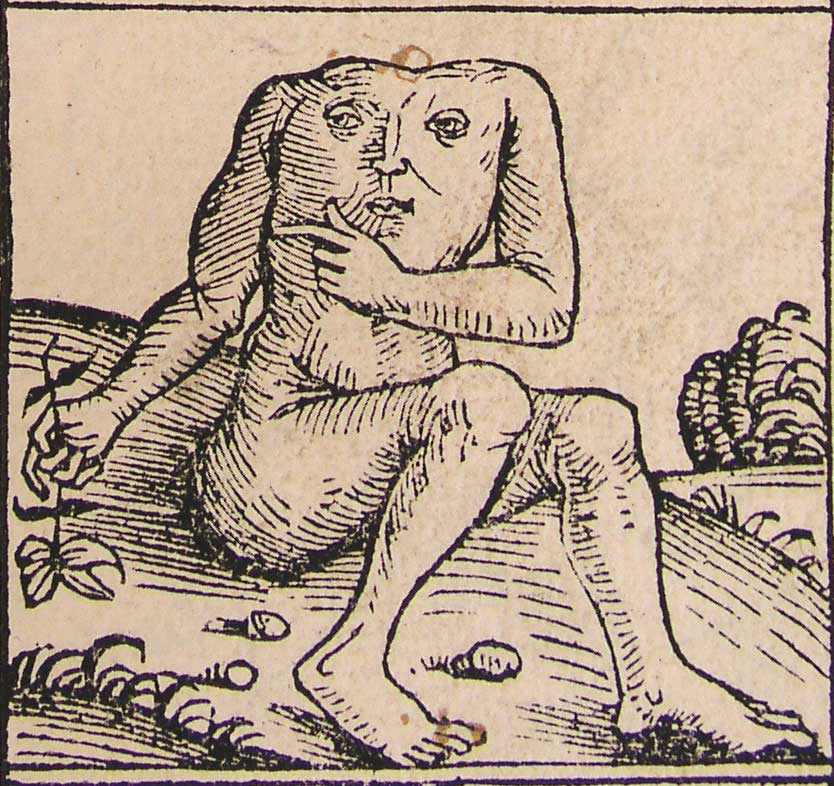
\includegraphics[width=.6\textwidth]{Figures/nuremberg-chronicles-strange-people-headless.jpg}
 
\caption{Figure from Hartmut Schedel's \emph{Liber Chronicarum}; Nuremberg, 1493}\label{fig-headless}
\end{figure}


\section*{\acknowledgmentsEN}

\largerpage
We would like to thank the participants of the workshop in Berlin for their fruitful discussions
that helped us to better understand the issues surrounding headedness and in particular our
(non-anonymous) reviewer, Stefan Müller, for his thoughtful comments on an earlier version of this
paper. 


\nocite{chapters/lander,chapters/salzmann,chapters/mueller,chapters/demske,chapters/korth,chapters/haider,chapters/raffelsiefen,chapters/noel,chapters/buecker,chapters/nolda}


\newpage

{\sloppy
\printbibliography[heading=subbibliography,notkeyword=this]
}
\end{document}



% en
%      <!-- Local IspellDict: en_GB-ise-w_accents -->
